% !TEX TS-program = pdflatex
% !TEX encoding = UTF-8 Unicode

% This is a simple template for a LaTeX document using the "article" class.
% See "book", "report", "letter" for other types of document.

\documentclass[11pt]{article} % use larger type; default would be 10pt

\usepackage[utf8]{inputenc} % set input encoding (not needed with XeLaTeX)

%%% PAGE DIMENSIONS
\usepackage{geometry} % to change the page dimensions
\geometry{a4paper} % or letterpaper (US) or a5paper or....

\usepackage{graphicx} % support the \includegraphics command and options

\usepackage{amssymb}
\usepackage{amsmath}
%%% PACKAGES
\usepackage{booktabs} % for much better looking tables
\usepackage{array} % for better arrays (eg matrices) in maths
\usepackage{paralist} % very flexible & customisable lists (eg. enumerate/itemize, etc.)
\usepackage{verbatim} % adds environment for commenting out blocks of text & for better verbatim
\usepackage{subfig} % make it possible to include more than one captioned figure/table in a single float
% These packages are all incorporated in the memoir class to one degree or another...

%%% HEADERS & FOOTERS
\usepackage{fancyhdr} % This should be set AFTER setting up the page geometry
\pagestyle{fancy} % options: empty , plain , fancy
\renewcommand{\headrulewidth}{0pt} % customise the layout...
\lhead{}\chead{}\rhead{}
\lfoot{}\cfoot{\thepage}\rfoot{}

%%% SECTION TITLE APPEARANCE
\usepackage{sectsty}
\allsectionsfont{\sffamily\mdseries\upshape} % (See the fntguide.pdf for font help)
% (This matches ConTeXt defaults)

%%% ToC (table of contents) APPEARANCE
\usepackage[nottoc,notlof,notlot]{tocbibind} % Put the bibliography in the ToC
\usepackage[titles,subfigure]{tocloft} % Alter the style of the Table of Contents
\renewcommand{\cftsecfont}{\rmfamily\mdseries\upshape}
\renewcommand{\cftsecpagefont}{\rmfamily\mdseries\upshape} % No bold!
\usepackage{graphicx}
\graphicspath{ {./pings/} }

\usepackage{amsmath}
\DeclareMathOperator*{\argmax}{arg\,max}
\DeclareMathOperator*{\argmin}{arg\,min}

\newcount\colveccount
\newcommand*\colvec[1]{
        \global\colveccount#1
        \begin{pmatrix}
        \colvecnext
}
\def\colvecnext#1{
        #1
        \global\advance\colveccount-1
        \ifnum\colveccount>0
                \\
                \expandafter\colvecnext
        \else
                \end{pmatrix}
        \fi
}

%%% END Article customizations

%%% The "real" document content comes below...

\title{Macro PS1}
\author{Michael B. Nattinger\footnote{I worked on this assignment with my study group: Alex von Hafften, Andrew Smith, and Ryan Mather. I have also discussed problem(s) with Emily Case, Sarah Bass, and Danny Edgel.}}

%\date{} % Activate to display a given date or no date (if empty),
         % otherwise the current date is printed 

\begin{document}
\maketitle
\section{Question 1}
\subsection{Part A}
\begin{align*}
V(A_t,c_{t-1}) = &\max_{c_t,A_{t+1}} u(c_t,c_{t-1}) + \beta V(A_{t+1},c_t)\\
&\text{s.t. } A_{t+1} = R(A_t - c_t)
\end{align*}

We can rewrite this as the following:

\begin{align}
V(A_t,c_{t-1}) = &\max_{c_t} u(c_t,c_{t-1}) + \beta V(R(A_t - c_t),c_t) \label{eqn:V1}%\\
%V(A_t,c_{t-1}) = &\max_{A_t} u\left(A_t - \frac{A_{t+1}}{R},c_{t-1}\right) + \beta V\left(A_{t+1},A_t - \frac{A_{t+1}}{R}\right) \label{eqn:V2}
\end{align}

To ensure the solution is unique, with a strictly increasing, strictly concave value function that is differentiable on the interior of the feasible set, we require the following assumptions:
\begin{itemize}
\item $(F1),(F2),(F3),(F4),(\Gamma 1),(\Gamma 2), (\Gamma 3)$ from lecture.
%\item $\lim_{k\rightarrow 0} u'(k,u) = \lim_{k\rightarrow 0} u'(u,k) = \infty$
%\item $\lim_{k\rightarrow \infty} u'(k,u) = \lim_{k\rightarrow \infty} u'(u,k) = 0$
\end{itemize}

Assuming the above conditions hold, we can solve the value function as it is written in (\ref{eqn:V1}) by taking a first order condition with respect to $c_t,$ and then applying the envelope theorem twice:
%\begin{align*}
%0 &=\frac{\partial u}{\partial c_t}(c_t,c_{t-1}) - R\beta \frac{\partial V}{\partial R(A_t - c_t)}(R(A_t - c_t),c_t) + \beta \frac{\partial V}{\partial c_t}(R(A_t - c_t),c_t)\\
%\frac{\partial V}{\partial R(A_t - c_t)}(R(A_t - c_t),c_t) &= 999\\
%\frac{\partial V}{\partial c_t}(R(A_t - c_t),c_t) &= \frac{\partial u}{\partial c_t}(c_{t+1},c_{t}) \\
%\Rightarrow \frac{\partial u}{\partial c_t}(c_t,c_{t-1}) + \beta () &= R\beta ()
%\end{align*}

\begin{align}
0&= u_1(c',c) + \beta (-RV_1(RA-Rc',c') + V_2(RA-Rc',c')) \label{eqn:FOC} \\
V_1(A,c) &= R\beta V_1(RA-Rc',c') \label{eqn:env1} \\
V_2(A,c) &= u_2(c',c) \label{eqn:env2}
\end{align}
Next, we can substitute in the envelope conditions (\ref{eqn:env1}), (\ref{eqn:env2}) into our first order condition (\ref{eqn:FOC}) to find an expression for $V_1,$ and substitute back into our initial first order condition (\ref{eqn:FOC}):
\begin{align*}
\Rightarrow 0 &= u_1(c',c) + \beta \left( -\frac{V_1(A,c)}{\beta} + u_2(c'',c')\right)
\end{align*}
\begin{align}
\Rightarrow V_1(A,c) &= u_1(c',c) + \beta u_2(c'',c') \label{eqn:redux}
\end{align}
We can now combine equations (\ref{eqn:FOC}), (\ref{eqn:env2}), (\ref{eqn:redux}) to yield the following:
\begin{align*}
 0&= u_1(c',c) + \beta(-R(u_1(c'',c') + \beta u_2(c''',c'')) + u_2(c'',c'))
\end{align*}
\begin{align}
\Rightarrow 0&= u_1(c',c) - \beta R u_1(c'',c') - \beta^2 R u_2(c''',c'') + \beta u_2(c'',c') \label{eqn:optcon}
\end{align}

Equation (\ref{eqn:optcon}) yields our optimality condition.

\subsection{Part B}
With the utility function as given, our value function becomes the following:
\begin{align*}
V(A,c) &= \max_{c'} log(c') + \gamma log(c) + \beta V(RA-Rc',c')
\end{align*}
The optimal choice $c'$ takes the form of the $\argmax$ of the optimization problem. 
\begin{align*}
c' &= \argmax_{c'}  log(c') + \gamma log(c) + \beta V(RA-Rc',c')\\
&= \argmax_{c'}  log(c') + \beta V(RA-Rc',c')\\
&=  \argmax_{c'}  log(c') + \beta \max_{c''}\{ log(c'') + \gamma log(c')  + \beta V(RA'-Rc'',c'')\} \\
&= \argmax_{c'}  (1+\beta \gamma) log(c') + \beta \max_{c''}\{ log(c'')   + \beta V(RA'-Rc'',c'')\} \\
%&=  \argmax_{c'}  log(c') + \gamma log(c) + \beta \max_{c''} log(c'') + \gamma log(c') + \beta V(RA-Rc'',c'') \\ %V(RA-Rc',c')
%&=  \argmax_{c'}  log(c') + \gamma log(c') + \gamma log(c) + \beta \max_{c''} log(c'')  + \beta V(RA-Rc'',c'') \\
%&=  \argmax_{c'}  log(c') + \gamma log(c') + \beta \max_{c''} log(c'')  + \beta V(RA-Rc'',c'') 
\end{align*}
\begin{equation}
\Rightarrow c' = \argmax_{c'}   log(c') + \beta \tilde{V}(RA-Rc') \label{eqn:vtilde}
\end{equation}

 This $\argmax$ is independent of c. Note that we have shown that the choice of $c_t$ not only does not depend on $c_{t-1},$ but is also equivalent to the choice of $c_t$ from a value function using standard log preferences ($\tilde{V}(A) = \max_{c} log(c) + \beta \tilde{V}(RA-Rc)$).

%We can rewrite this Bellman equation as the following, which will preserve the choice of $c'$:
%\begin{align*}
%V(A) &= \max_{A'} (1+\gamma)log\left(\frac{A'}{R} - A \right)  + \beta V(A')
%\end{align*}
%Taking FOC's,
%\begin{align*}
%0 &= \frac{1+\gamma}{R\left(\frac{A'}{R} - A \right)} +\beta V'(A')\\
%V'(A) &= -\frac{1+\gamma}{\left(\frac{A'}{R} - A \right)} \\
%\Rightarrow  \frac{1+\gamma}{R\left(\frac{A'}{R} - A \right)} &=\beta \frac{1+\gamma}{\left(\frac{A''}{R} - A' \right)}\\
%\Rightarrow \left(\frac{A''}{R} - A' \right) &= \beta R\left(\frac{A'}{R} - A \right)\\
%\Rightarrow A'' &= A'(1+\beta)R - \beta R^2 A
%\end{align*}

Now we will solve for our optimality conditions. Applying (\ref{eqn:optcon}) to our new utility function yields the following:
\begin{align*}
\beta R (c'')^{-1} + \gamma \beta^2 R (c'')^{-1}&=(c')^{-1} + \gamma \beta (c')^{-1}\\
\Rightarrow c' \beta R (1+\gamma \beta) &= c''(1+\gamma \beta)
\end{align*}
\begin{align}
\Rightarrow c'\beta R &= c'' \label{eqn:euler}
\end{align}
Equation (\ref{eqn:euler}) yields our Euler conditions.

Recall that, due to properties of argmax, our choice of $c_t$ is equivalent to the choice of $c_t$ from a different value function, $\tilde{V}(A) = \max_{A'} log(A'/R- A) + \beta \tilde{V}(A')$. We will show that this implies that we will save a constant portion of our assets.

Given $A_t$ we will choose some consumption amount $c_t$ which will correspond to some ratio of $A_t$. Let $c_t = aA_t$ for some $a \in (0,1)$. Then, we can combine this fact with $(\ref{eqn:euler})$ to form a guess for our value function: $\tilde{V}(A) = \sum_{i=0}^n \beta^i log((\beta R)^iaA)$. We can plug this into our formulation for the value function:

\begin{align*}
 \sum_{i=0}^n \beta^i log((\beta R)^iaA) = \max_{A'} log(A'/R- A) + \beta \sum_{i=0}^{\infty} \beta^i log((\beta R)^iaA')
\end{align*}

Taking FOCs:
\begin{align*}
\frac{1}{RA-A'} &= \beta\sum_{i=0}^{\infty} \beta^{i}\frac{(\beta R)^{i}a}{(\beta R)^{i}aA'}\\
\Rightarrow \frac{A'}{aRA} &= \frac{\beta}{1-\beta}\\
\Rightarrow \frac{RA(1-a)}{aRA} &= \frac{\beta}{1-\beta}\\
\Rightarrow \frac{(1-a)}{a} &= \frac{\beta}{1-\beta}\\
\Rightarrow a &= 1-\beta
\end{align*}

Therefore, the optimal policy function is to consume $1-\beta$ of your assets in each period and to save $\beta$ of your assets.
 %This implies that the optimal saving policy is to save a current fraction of current assets. %show via guess and verify?

%\begin{align*}
%V(k,c) &= \max_{k'} log(A-k'/R) + \gamma log(c) + \beta V(k',A-k'/R)
%&= 
%\end{align*}

%Given a set of assets in an initial period, $A_1$, $c_{t+1}  = \beta R c_t$ $\forall t \in \mathbb{N}$. 
%With the utility function as given, our value function becomes the following:
%\begin{align*}
%V(A,c) &= \max_{c'} log(c') + \gamma log(c) + \beta V(RA-Rc',c')
%\end{align*}
%The optimal choice $c'$ takes the form of the $\argmax$ of the optimization problem. 
%\begin{align*}
%c' &= \argmax_{c'}  log(c') + \gamma log(c) + \beta V(RA-Rc',c')\\
%&=  \argmax_{c'}  log(c') + \gamma log(c) + \beta \max_{c''} log(c'') + \gamma log(c') + \beta V(RA-Rc'',c'') \\ %V(RA-Rc',c')
%&=  \argmax_{c'}  log(c') + \gamma log(c') + \gamma log(c) + \beta \max_{c''} log(c'')  + \beta V(RA-Rc'',c'') \\
%&=  \argmax_{c'}  log(c') + \gamma log(c') + \beta \max_{c''} log(c'')  + \beta V(RA-Rc'',c'') 
%\end{align*}
% This $\argmax$ is independent of c
%\begin{align*}
%
%\end{align*}
%I think that doesn't work - taking another crack at it here

%Instead we will use the value function as it is written in (\ref{eqn:V2}) by taking a first order condition with respect to $A_{t+1},$ and then applying the envelope theorem twice:
%\begin{align*}
%0 &=\frac{-1}{R}\frac{\partial u}{\partial A_t - \frac{A_{t+1}}{R}}\left(A_t - \frac{A_{t+1}}{R},c_{t-1}\right) + \beta \frac{\partial V}{\partial A_{t+1}}\left(A_{t+1},A_t - \frac{A_{t+1}}{R}\right) - \frac{\beta}{R} \frac{\partial V}{\partial A_t - \frac{A_{t+1}}{R}}\left(A_{t+1},A_t - \frac{A_{t+1}}{R}\right)\\
%&\frac{\partial V}{\partial R(A_t - c_t)}(R(A_t - c_t),c_t) = 999\\
%&\frac{\partial V}{\partial c_t}(R(A_t - c_t),c_t) = \frac{\partial u}{\partial c_t}(c_{t+1},c_{t}) \\
%&\Rightarrow \frac{\partial u}{\partial c_t}(c_t,c_{t-1}) + \beta () = R\beta ()
%\end{align*}

\subsection{Part C}

No, in general this will not hold. The only reason why this held in part B is that the utility function given to us was a seperable utility function. 

\section{Question 2}
\subsection{Part A}
The sequence problem is to maximize profits:
\begin{align*}
\max_{\{ x_t\}_{i=0}^{\infty}} \sum_{i=0}^{\infty}\left( \frac{1}{1+r} \right)^{t}\left( ax_t - \frac{b}{2}x_t^2 - \frac{c}{2}(x_{t+1}-x_t)^2\right)
\end{align*}

We can rewrite this as a bellman equation in the following way:

\begin{align}
V(x) =\max_{y} ax - \frac{b}{2}x^2 - \frac{c}{2}(y-x)^2 + \delta V(y) \label{eqn:bell}
\end{align}

We can rewrite this as follows:

\begin{align}
T(v)(x) =\max_{y} ax - \frac{b}{2}x^2 - \frac{c}{2}(y-x)^2 + \delta v(y) \label{eqn:bellT}
\end{align}

where the fixed point of our $T$ operator in (\ref{eqn:bellT}) is the solution to the Bellman equation in (\ref{eqn:bell}).

\subsection{Part B}

Let $L<0$ be arbitrary. If we set $y=0,x<\frac{L}{a}$ then $F(x,y) = ax -\frac{b}{2}x^2 - \frac{c}{2}(y-x)^2 \leq ax<L$ so $F$ is unbounded below.

This $F$ function is of the form of a polynomial with limits of negative infinity in all directions, so we can find the global maximum by taking first order conditions:
 \begin{align*}
0 &= a - bx + c(y-x)\\
0 &= -c(y-x) \Rightarrow y-x = 0 \Rightarrow y=x\\
\Rightarrow y = x &= \frac{a}{b}\\
F\left( \frac{a}{b},\frac{a}{b} \right) &= a\left(\frac{a}{b}\right) - \frac{b}{2}\left( \frac{a}{b}\right)^2 - 0\\
&= \frac{a^2}{2b}
\end{align*}

Therefore, the maximum value $F$ can take is $\frac{a^2}{2b}$

We can find bounds on $\hat{v}$ in the following way:

\begin{align*}
\hat{v} &= \frac{a^2}{2b} + \delta \hat{v}\\
\Rightarrow \hat{v} &= \frac{a^2}{2b(1-\delta)} 
\end{align*}

\subsection{Part C}
\begin{align*}
T\hat{v}(x) &= \max_{y} ax - \frac{b}{2}x^2 - \frac{c}{2}(y-x)^2 + \delta \hat{v}\\
0 &= -c(y-x) \Rightarrow y=x,\\
\Rightarrow T\hat{v}(x) &= ax -\frac{b}{2}x^2 +\delta \hat{v} \\
&\leq \frac{a^2}{2b} +\delta \frac{a^2}{2b(1-\delta)} = \frac{a^2}{2b(1-\delta)}\\
&= \hat{v}.
\end{align*}

\subsection{Part D}
We showed the base case of the induction in Part C. Now we will show the induction step.

Assume that $T^n\hat{v}(x)$ takes the form $T^n\hat{v}(x) = \alpha_n x - \frac{1}{2}\beta_n x^2 + \gamma_n.$ Then,
\begin{align*}
T^{n+1}\hat{v} (x) &= \max_y ax - \frac{b}{2}x^2 - \frac{c}{2}(y-x)^2 + \delta (\alpha_n y - \frac{1}{2}\beta_n y^2 + \gamma_n)\\
\Rightarrow 0 &= cx - cy + \delta \alpha_n - \delta \beta_n y \\
\Rightarrow y &= \left(\frac{cx + \delta \alpha_n}{c+\delta \beta_n}\right)\\
T^{n+1}\hat{v} (x) &= ax - \frac{b}{2}x^2 - \frac{c}{2}\left( \left(\frac{cx + \delta \alpha_n}{c+\delta \beta_n}\right)-x\right)^2 + \delta \left(\alpha_n  \left(\frac{cx + \delta \alpha_n}{c+\delta \beta_n}\right) - \frac{1}{2}\beta_n  \left(\frac{cx + \delta \alpha_n}{c+\delta \beta_n}\right)^2 + \gamma_n\right)\\
&=  ax - \frac{b}{2}x^2 - \frac{c \delta^2 \alpha_n^2}{2(c+\delta \beta_n)^2} +\frac{c\delta^2\alpha_n \beta_n}{(c+\delta \beta_n)^2}x - \frac{c \delta^2 \beta_n^2}{2(c+\delta \beta_n)^2}x^2  + \frac{\delta^2 \alpha_n^2}{c+\delta \beta_n} + \frac{ \delta \alpha_n c }{c+\delta \beta_n}x \\ &- \frac{1}{2}\frac{\delta \beta_n c^2x^2}{(c+\delta \beta_n)^2} -  \frac{1}{2}\frac{\delta \alpha_n c x}{(c+\delta \beta_n)^2} - \frac{1}{2}\frac{\delta^2 \alpha_n^2}{(c+\delta \beta_n)^2}+ \delta \gamma_n \\
&= \left( a + \frac{2c\delta^2\alpha_n \beta_n}{(c+\delta \beta_n)^2}  + \frac{ \delta \alpha_n c }{c+\delta \beta_n}  -  \frac{1}{2}\frac{\delta \alpha_n c}{(c+\delta \beta_n)^2}\right) x \\
&- \frac{1}{2}\left( b +  \frac{c \delta^2 \beta_n^2}{(c+\delta \beta_n)^2} + \frac{\delta \beta_n c^2}{(c+\delta \beta_n)^2} \right) x^2 \\
&+\left( - \frac{c \delta^2 \alpha_n^2}{2(c+\delta \beta_n)^2} + \frac{\delta^2 \alpha_n^2}{c+\delta \beta_n} - \frac{1}{2}\frac{\delta^2 \alpha_n^2}{(c+\delta \beta_n)^2}+ \delta\gamma_n\right)\\
%&= \left(a +\frac{c \delta \alpha_n}{c+ \beta_n \delta} \right) x - \frac{1}{2} \left( b + \frac{c \beta_n \delta }{c+ \beta_n \delta} \right)x^2 + \left( \delta \gamma + (1/2)\frac{\alpha_n^2 \delta^2}{c+\beta_n \delta} \right) \\
&=\alpha_{n+1} x -\frac{1}{2}\beta_{n+1}x^2 + \gamma_{n+1}.
%y=x \Rightarrow T^{n+1}\hat{v} (x) &= ax - \frac{b}{2}x^2 + \delta \alpha_n x - \delta \frac{1}{2}\beta_n x^2 + \delta \gamma_n\\
%&= (a+\delta \alpha_n) x - \frac{b + \delta \beta_n}{2}x^2 +\delta \gamma_n\\
%&= \alpha_{n+1} x - \frac{1}{2}\beta_{n+1} x^2 + \gamma_{n+1}
\end{align*}


\subsection{Part E}
To find the fixed point, we find the steady state of the three difference equations. This yields the following results: $\alpha_n = a$, $\beta_n = b$

\begin{align*}
\tilde{V} &= \lim_{n\rightarrow \infty} T^n \hat{v} = \frac{a}{1-\delta}x - \frac{1}{2}\frac{b}{1-\delta}x^2.\\
T\tilde{V} &= \max_{y} ax - \frac{b}{2}x^2 - \frac{c}{2}(y-x)^2 + \delta \frac{a}{1-\delta}x - \frac{1}{2}\frac{b}{1-\delta}x^2,\\
y=x\Rightarrow T\tilde{V} &=  ax - \frac{b}{2}x^2 + \delta \frac{a}{1-\delta}x - \frac{1}{2}\frac{b}{1-\delta}x^2\\
&= \frac{a}{1-\delta}x - \frac{1}{2}\frac{b}{1-\delta}x^2\\
&= \tilde{V}.
\end{align*}
Therefore, the limit function $\tilde{V}$ satisfies the Bellman equation.
\section{Question 3}
\subsection{Part A}
The Bellman equation takes the following form:
\begin{align*}
V(k) &= \max_{k'} \pi (k) - \gamma(k' - (1-\delta)k) + \frac{1}{R}V(k')
\end{align*}

We maximize by taking first order conditions and applying the envelope theorem:
\begin{align*}
\gamma' (k' - (1-\delta)k) &= \frac{1}{R} V'(k')\\%\left( \pi'(k') + (1-\delta) \gamma'(k'' - (1-\delta)k') \right)\\
V'(k) = \pi'(k) + (1-\delta) \gamma ' (k' - (1-\delta)k)\\
\Rightarrow \pi '(k') + (1-\delta) \gamma ' (k'' - (1-\delta)k')&= R \gamma'(k' - (1-\delta)k).
\end{align*}

The above equation forms our condition for maximization.

\subsection{Part B}
Letting $k = k' = k'' = \bar{k},$ we know that $\bar{I} = \delta \bar{k}$ and, moreover, we can rewrite our conditions for optimization in the following way:

\begin{align*}
\pi '(\bar{k}) + (1-\delta) \gamma '(\bar{I}) &= R \gamma'(\bar{I}))\\
\Rightarrow \pi'(\bar{k}) &= (R-1 + \delta)\gamma'(\delta \bar{k})\\
\Rightarrow \frac{ \pi'(\bar{k})}{\gamma'(\delta \bar{k})} &= (R-1+ \delta)
\end{align*}
 By the strict convexity of $\gamma$ and strict concavity of $\pi$, in addition to our Inada conditions, the solution exists and is unique.

If $R$ were to increase, the steady state level of $\pi'(\bar{k})$ would increase, resulting in a reduction in $\bar{k}$, and since $\bar{I} = \delta \bar{k}$, $\bar{I}$ will fall as well. An economic intuition of this is that an increase in the interest rate reduces capital levels and investment spending in the long run.

\subsection{Part C}
Our optimality conditions become:
\begin{align*}
-(k'-k^{*}) &= R(k' - (1-\delta)k) - (1-\delta)(I')\\
\Rightarrow -(k'-k^{*}) &= RI -(1-\delta)I'
\end{align*}
This, in addition to our law of motion for capital, $k' = I + (1-\delta)k$, forms the difference equations for capital and investment.

We will now derive our phase diagrams. $\Delta k = 0$ implies that $I = \delta k$. $\Delta I = 0$ implies that $-(I + (1-\delta)k - k^{*}) = RI - (1-\delta)I \Rightarrow I = \frac{k^{*}}{R+\delta} - \frac{(1-\delta)}{R+\delta}k$. If we are above $\Delta k = 0$ then we are investing more than the rate of depreciation so capital goes to the right. If we are to the right of $\Delta I=0$ then we are underinvesting so I will increase. We can draw the phase diagram below.

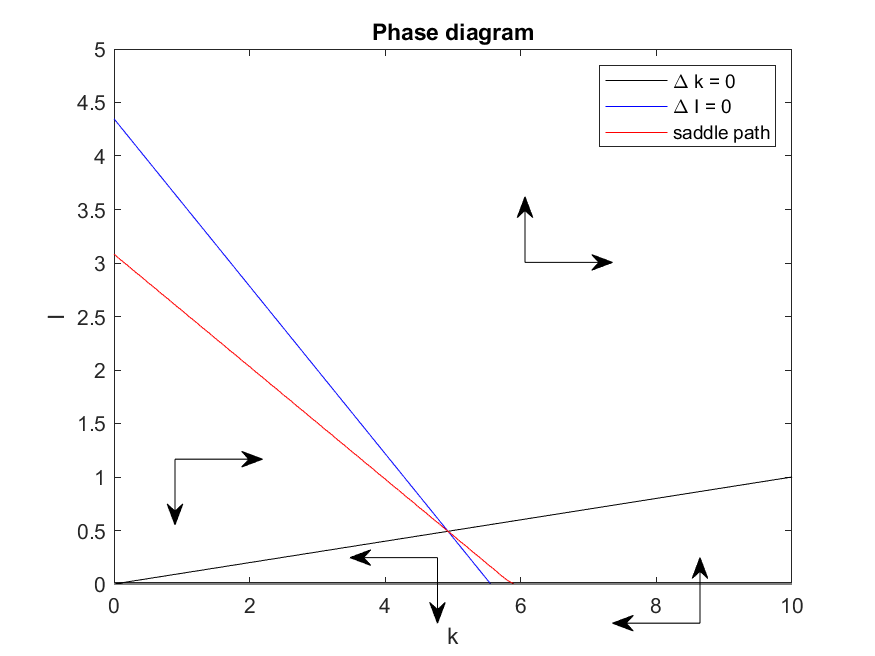
\includegraphics{phase3}

If the interest rate were to rise, there would not be an initial change in the capital level as $k'$ is already exactly determined by $I,k$. Investment spending would instead adjust and would immediately decrease. Specifically, investment spending would decrease so as to move to the new saddle path. The system would then follow the new saddle path to the new steady state. We plot this transition below.

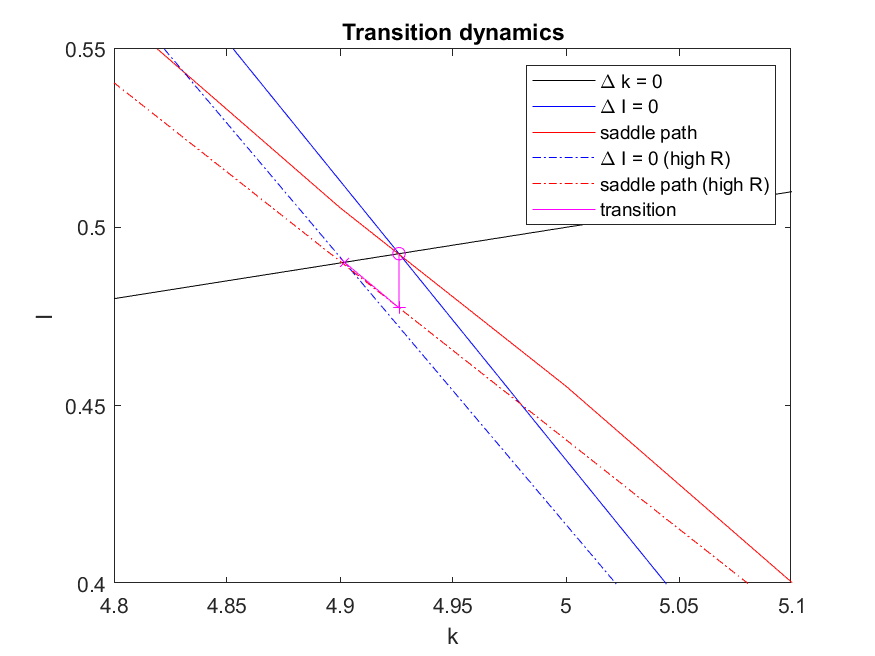
\includegraphics{transition3}

In the above figure, we begin at the original steady state. When the  interest rate rises, investment falls from the magenta o to the magenta $+$. Then, the system proceeds to follow the new saddle path to the new steady state, eventually converging to the magenta x.

\section{Question 4}
\subsection{Part A}
%The Bellman equation takes the following form:
%\begin{align*}
%V(k) =\max_{c} \frac{1}{1-\gamma} (c G^{\eta})^{1-\gamma} + \beta V((1-\delta)k +f(k) - c)
%\end{align*}
%
%We will find the conditions for maximization by taking first order conditions and applying the envelope conditions:
%
%\begin{align*}
%c^{-\gamma}(G^{\eta})^{1-\gamma} - \beta V'((1-\delta)k +f(k) - c) &= 0\\
%V'(k) &= \beta V'((1-\delta)k + f(k) - c) (1-\delta + f'(k))\\
%\Rightarrow c^{-\gamma}(G^{\eta})^{1-\gamma} &= \frac{V'(k)}{1-\delta + f'(k)} \\
%\Rightarrow V'(k) &=  c^{-\gamma}(G^{\eta})^{1-\gamma} (1-\delta + f'(k))\\
%\Rightarrow c^{-\gamma}(G^{\eta})^{1-\gamma} &= \beta c^{-\gamma}(G^{\eta})^{1-\gamma} (1-\delta + f'((1-\delta)k +f(k) - c))\\
%\Rightarrow \frac{1}{\beta} &= 1-\delta + f'((1-\delta)k +f(k) - c)\\
%\Rightarrow f'((1-\delta)k +f(k) - c) &= \frac{1}{\beta} + \delta - 1.
%\end{align*}
%\subsection{Part B}
%
%Yes, we can still have a unique steady state regardless of g. We can solve for $\bar{c},\bar{k}$ as follows:
%\begin{align*}
%\bar{c}&= (1-\delta)\bar{k}  + f(\bar{k}) - f'^{-1}( \frac{1}{\beta} + \delta - 1)\\
%\delta \bar{k} - f(\bar{k}) = - \bar{c}
%\end{align*}
%The above equations form 2 equations in 2 unknowns which pin down our steady state values.
%\subsection{Part C}
We will write our Bellman equation in the following form:
\begin{align}
V(k) = \max_{k'} (((1-\delta) k + f(k) - k')G^{\eta})^{1-\gamma}/(1-\gamma) + \beta V(k') \label{eqn:bellk}
\end{align}

By taking first order conditions and applying the envelope theorem, we get the following:
\begin{align*}
\beta V'(k') &=((1-\delta) k + f(k) - k')^{-\gamma}G^{\eta(1-\gamma)}\\
V'(k') &=((1-\delta) k' + f(k') - k'')^{-\gamma}(G')^{\eta(1-\gamma)}((1-\delta) + f'(k'))\\
\Rightarrow ((1-\delta) k + f(k) - k')^{-\gamma}G^{\eta(1-\gamma)} &=\beta ((1-\delta) k' + f(k') - k'')^{-\gamma}(G')^{\eta(1-\gamma)}((1-\delta) + f'(k'))\\
\end{align*}
\begin{align}
\Rightarrow \left( \frac{c'}{c}\right)^{\gamma} &= \left( \frac{G'}{G}\right)^{\eta(1-\gamma)}\beta ((1-\delta) + f'(k')) \label{eqn:optconk}
\end{align}

Equation (\ref{eqn:optconk}) along with the identity $k' = (1-\delta)k + f(k) - c$ form our difference equations for $k',c'$ (2 equations, 2 variables).

\subsection{Part B}

If government spending grows at a constant rate, $g$, then we can find steady state values $\bar{k},\bar{c}$ from our difference equations:

\begin{align*}
1 = g^{\eta(1-\gamma)}\beta((1-\delta) + f'(\bar{k}))\\
\Rightarrow \bar{k} = f'^{-1}(g^{-\eta(1-\gamma)}\beta^{-1} - 1+ \delta)\\
\Rightarrow \bar{c} = f(\bar{k}) - \delta \bar{k}.
\end{align*}

Since $f$ is strictly concave with the Inada conditions listed, the steady state exists and is unique.

\subsection{Part C}
Our identity $k' = (1-\delta)k + f(k) - c$ shows that in the period where $g$ increases, the level of capital was already predetermined in the period before so it will remain at its initial level. Our value for $c$ then makes the initial adjustment, and as $g$ increases then $c'/c$ increases, so (assuming consumption is positive), consumption increases. The increase in consumption results in lower capital in the next period. This lower capital increases $f'(k)$, resulting in a further increase in consumption. Eventually, the system will approach its new steady state. The new steady state value for capital will be higher as an increase in $g$ will result in an increase in $f'^{-1}$, and therefore an increase in $\bar{k}.$ The higher value for the steady state of capital has an indeterminate effect on the steady state of consumption as it will increase the $f(\bar{k})$ term but decrease the $-\delta \bar{k}$ term. The more an agent prefers government spending ($\eta$), the more the steady state capital level will move, and the larger the move in capital the more the $-\delta \bar{k}$ term moves relative to $f(\bar{k})$ due to the concavity of $f$. Thus, for higher values of $\eta$, the steady state consumption levels will drop while for lower values of $\eta$ the steady state consumption levels will increase. We can show this numerically via Matlab, which I will show below.

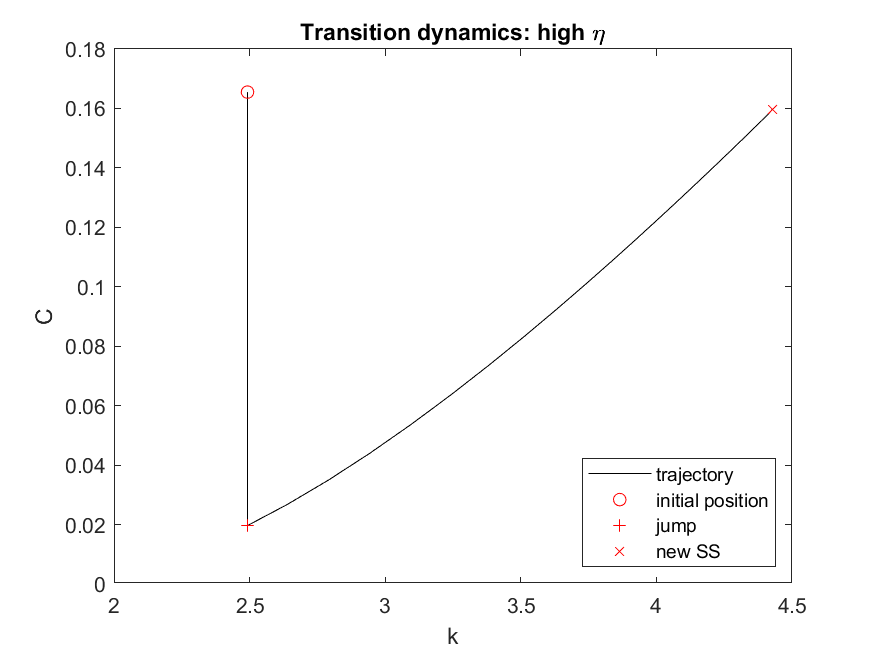
\includegraphics{higheta}

The above figure shows the transition from an increase in $g$ for a relatively high value of $\eta$. Since the $-\delta \bar{k}$ term dominates the $f(\bar{k})$ term in this case, the steady state level of consumption falls. We will show below that this is not always the case, and that for lower levels of $\eta$ the steady state consumption level can increase.

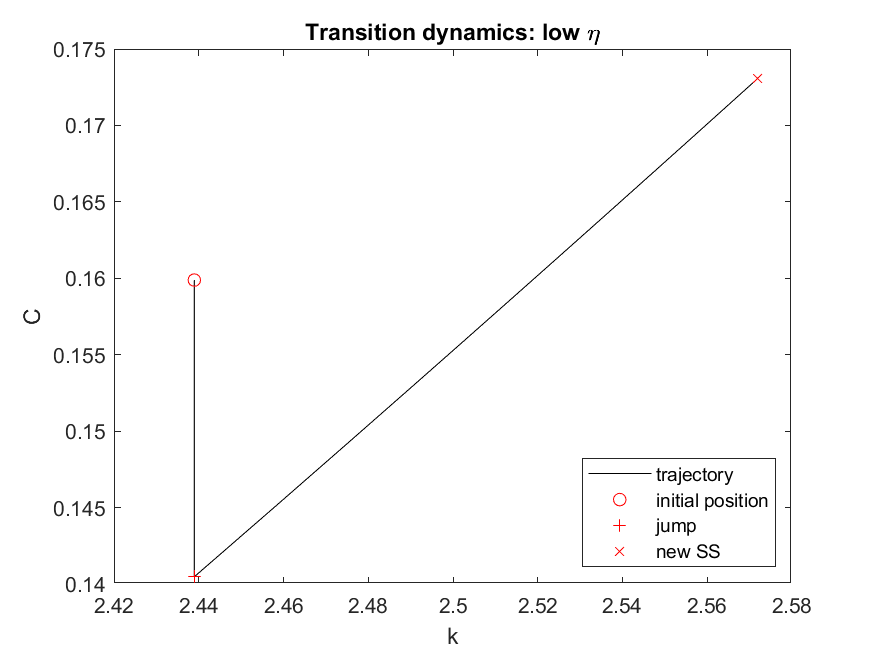
\includegraphics{loweta}

This figure, which is identical in parameterization from the previous figure except for a lower value of $\eta$, shows that it is possible for the new steady state level of consumption to increase.

An economic interpretation of our findings are that an increase in government spending reduces consumption spending in the short run, increases capital in the long run, but has an indeterminate long run effect on consumption.

\end{document}
